% results_section.tex - preliminary results (mid-semester). Numbers: % numbers.tex - GENERATED by paper/make_numbers.py from results/; do not edit.
\newcommand{\NumBandMax}{50\,\%}
\newcommand{\NumBandMin}{18\,\%}
\newcommand{\NumCmsisMax}{31.4}
\newcommand{\NumCmsisMedian}{17.6}
\newcommand{\NumCmsisMin}{5.9}
\newcommand{\NumCnnFpOverIntMax}{30.5}
\newcommand{\NumCnnFpOverIntMin}{5.4}
\newcommand{\NumConfigs}{68}
\newcommand{\NumFeROneKcyc}{34.4}
\newcommand{\NumFeROneUs}{538}
\newcommand{\NumFeRThreeKcyc}{145.9}
\newcommand{\NumFeRThreeUs}{2280}
\newcommand{\NumFeRTwoKcyc}{124.0}
\newcommand{\NumFeRTwoUs}{1938}
\newcommand{\NumFeRZeroKcyc}{9.3}
\newcommand{\NumFeRZeroUs}{145}
\newcommand{\NumFlashMaxKB}{324}
\newcommand{\NumFrontPOneEtoe}{11}
\newcommand{\NumFrontPOneInf}{11}
\newcommand{\NumFrontPThreeEtoe}{4}
\newcommand{\NumFrontPThreeInf}{4}
\newcommand{\NumFrontPTwoEtoe}{8}
\newcommand{\NumFrontPTwoInf}{9}
\newcommand{\NumFstarHi}{0.489}
\newcommand{\NumFstarHiModel}{\texttt{dt-r2-d6-fp32}}
\newcommand{\NumFstarLo}{0.032}
\newcommand{\NumFstarLoModel}{\texttt{cnn-r0-w025d2-int8qat}}
\newcommand{\NumFwBundles}{4}
\newcommand{\NumFwBundlesLink}{4}
\newcommand{\NumFwFlashMaxKB}{904}
\newcommand{\NumFwModels}{60}
\newcommand{\NumFwRamMaxKB}{186}
\newcommand{\NumHvExclPOneEtoeCNN}{0.000}
\newcommand{\NumHvExclPOneEtoeDT}{0.008}
\newcommand{\NumHvExclPOneEtoeMLP}{0.001}
\newcommand{\NumHvExclPOneEtoeRF}{0.000}
\newcommand{\NumHvExclPOneInfCNN}{0.000}
\newcommand{\NumHvExclPOneInfDT}{0.046}
\newcommand{\NumHvExclPOneInfMLP}{0.001}
\newcommand{\NumHvExclPOneInfRF}{0.002}
\newcommand{\NumHvExclPThreeEtoeCNN}{0.000}
\newcommand{\NumHvExclPThreeEtoeDT}{0.184}
\newcommand{\NumHvExclPThreeEtoeMLP}{0.000}
\newcommand{\NumHvExclPThreeEtoeRF}{0.031}
\newcommand{\NumHvExclPThreeInfCNN}{0.000}
\newcommand{\NumHvExclPThreeInfDT}{0.198}
\newcommand{\NumHvExclPThreeInfMLP}{0.000}
\newcommand{\NumHvExclPThreeInfRF}{0.043}
\newcommand{\NumHvExclPTwoEtoeCNN}{0.000}
\newcommand{\NumHvExclPTwoEtoeDT}{0.001}
\newcommand{\NumHvExclPTwoEtoeMLP}{0.000}
\newcommand{\NumHvExclPTwoEtoeRF}{0.057}
\newcommand{\NumHvExclPTwoInfCNN}{0.000}
\newcommand{\NumHvExclPTwoInfDT}{0.035}
\newcommand{\NumHvExclPTwoInfMLP}{0.000}
\newcommand{\NumHvExclPTwoInfRF}{0.068}
\newcommand{\NumHvPOneEtoeCNN}{0.359}
\newcommand{\NumHvPOneEtoeDT}{1.257}
\newcommand{\NumHvPOneEtoeMLP}{0.488}
\newcommand{\NumHvPOneEtoeRF}{1.259}
\newcommand{\NumHvPOneInfCNN}{0.262}
\newcommand{\NumHvPOneInfDT}{1.259}
\newcommand{\NumHvPOneInfMLP}{0.429}
\newcommand{\NumHvPOneInfRF}{1.224}
\newcommand{\NumHvPThreeEtoeCNN}{0.342}
\newcommand{\NumHvPThreeEtoeDT}{0.952}
\newcommand{\NumHvPThreeEtoeMLP}{0.454}
\newcommand{\NumHvPThreeEtoeRF}{0.859}
\newcommand{\NumHvPThreeInfCNN}{0.250}
\newcommand{\NumHvPThreeInfDT}{0.962}
\newcommand{\NumHvPThreeInfMLP}{0.398}
\newcommand{\NumHvPThreeInfRF}{0.858}
\newcommand{\NumHvPTwoEtoeCNN}{0.341}
\newcommand{\NumHvPTwoEtoeDT}{1.109}
\newcommand{\NumHvPTwoEtoeMLP}{0.463}
\newcommand{\NumHvPTwoEtoeRF}{1.230}
\newcommand{\NumHvPTwoInfCNN}{0.249}
\newcommand{\NumHvPTwoInfDT}{1.108}
\newcommand{\NumHvPTwoInfMLP}{0.402}
\newcommand{\NumHvPTwoInfRF}{1.192}
\newcommand{\NumNFrontPOneEtoeCNN}{0}
\newcommand{\NumNFrontPOneEtoeDT}{3}
\newcommand{\NumNFrontPOneEtoeMLP}{5}
\newcommand{\NumNFrontPOneEtoeRF}{3}
\newcommand{\NumNFrontPOneInfCNN}{0}
\newcommand{\NumNFrontPOneInfDT}{3}
\newcommand{\NumNFrontPOneInfMLP}{5}
\newcommand{\NumNFrontPOneInfRF}{3}
\newcommand{\NumNFrontPThreeEtoeCNN}{0}
\newcommand{\NumNFrontPThreeEtoeDT}{2}
\newcommand{\NumNFrontPThreeEtoeMLP}{0}
\newcommand{\NumNFrontPThreeEtoeRF}{2}
\newcommand{\NumNFrontPThreeInfCNN}{0}
\newcommand{\NumNFrontPThreeInfDT}{2}
\newcommand{\NumNFrontPThreeInfMLP}{0}
\newcommand{\NumNFrontPThreeInfRF}{2}
\newcommand{\NumNFrontPTwoEtoeCNN}{1}
\newcommand{\NumNFrontPTwoEtoeDT}{2}
\newcommand{\NumNFrontPTwoEtoeMLP}{0}
\newcommand{\NumNFrontPTwoEtoeRF}{5}
\newcommand{\NumNFrontPTwoInfCNN}{1}
\newcommand{\NumNFrontPTwoInfDT}{3}
\newcommand{\NumNFrontPTwoInfMLP}{0}
\newcommand{\NumNFrontPTwoInfRF}{5}
\newcommand{\NumNModelsCost}{68}
\newcommand{\NumPOneBest}{1.000}
\newcommand{\NumPOneBestModel}{\texttt{mlp-r3-h32-fp32}}
\newcommand{\NumPOneCNNBest}{1.000}
\newcommand{\NumPOneCNNBestModel}{\texttt{cnn-r0-w200d4-int8qat}}
\newcommand{\NumPOneCNNBestStd}{0.000}
\newcommand{\NumPOneCNNMedian}{0.999}
\newcommand{\NumPOneDTBest}{0.989}
\newcommand{\NumPOneDTBestModel}{\texttt{dt-r2-d12-fp32}}
\newcommand{\NumPOneDTBestStd}{0.001}
\newcommand{\NumPOneDTMedian}{0.959}
\newcommand{\NumPOneLeakPct}{98.1\,\%}
\newcommand{\NumPOneMLPBest}{1.000}
\newcommand{\NumPOneMLPBestModel}{\texttt{mlp-r3-h64-int8}}
\newcommand{\NumPOneMLPBestStd}{0.000}
\newcommand{\NumPOneMLPMedian}{1.000}
\newcommand{\NumPOneRFBest}{0.997}
\newcommand{\NumPOneRFBestModel}{\texttt{rf-r2-t25d10-fp32}}
\newcommand{\NumPOneRFBestStd}{0.001}
\newcommand{\NumPOneRFMedian}{0.965}
\newcommand{\NumPOneTest}{1{,}402}
\newcommand{\NumPOneTrain}{6{,}542}
\newcommand{\NumPOneVal}{1{,}402}
\newcommand{\NumPThreeBest}{0.623}
\newcommand{\NumPThreeBestModel}{\texttt{rf-r2-t25d6-fp32}}
\newcommand{\NumPThreeCNNBest}{0.612}
\newcommand{\NumPThreeCNNBestModel}{\texttt{cnn-r0-w025d2-int8qat}}
\newcommand{\NumPThreeCNNBestStd}{0.162}
\newcommand{\NumPThreeCNNMedian}{0.577}
\newcommand{\NumPThreeDTBest}{0.584}
\newcommand{\NumPThreeDTBestModel}{\texttt{dt-r2-d6-fp32}}
\newcommand{\NumPThreeDTBestStd}{0.216}
\newcommand{\NumPThreeDTMedian}{0.557}
\newcommand{\NumPThreeMLPBest}{0.608}
\newcommand{\NumPThreeMLPBestModel}{\texttt{mlp-r2-h64-fp32}}
\newcommand{\NumPThreeMLPBestStd}{0.252}
\newcommand{\NumPThreeMLPMedian}{0.592}
\newcommand{\NumPThreeRFBest}{0.623}
\newcommand{\NumPThreeRFBestModel}{\texttt{rf-r2-t25d6-fp32}}
\newcommand{\NumPThreeRFBestStd}{0.207}
\newcommand{\NumPThreeRFMedian}{0.516}
\newcommand{\NumPThreeTest}{1{,}542}
\newcommand{\NumPThreeTrain}{5{,}326}
\newcommand{\NumPThreeVal}{941}
\newcommand{\NumPTwoBest}{0.963}
\newcommand{\NumPTwoBestModel}{\texttt{cnn-r0-w100d4-int8qat}}
\newcommand{\NumPTwoCNNBest}{0.963}
\newcommand{\NumPTwoCNNBestModel}{\texttt{cnn-r0-w100d4-int8qat}}
\newcommand{\NumPTwoCNNBestStd}{0.053}
\newcommand{\NumPTwoCNNMedian}{0.924}
\newcommand{\NumPTwoDTBest}{0.902}
\newcommand{\NumPTwoDTBestModel}{\texttt{dt-r1-d8-fp32}}
\newcommand{\NumPTwoDTBestStd}{0.054}
\newcommand{\NumPTwoDTMedian}{0.800}
\newcommand{\NumPTwoMLPBest}{0.949}
\newcommand{\NumPTwoMLPBestModel}{\texttt{mlp-r3-h128-int8}}
\newcommand{\NumPTwoMLPBestStd}{0.074}
\newcommand{\NumPTwoMLPMedian}{0.905}
\newcommand{\NumPTwoRFBest}{0.962}
\newcommand{\NumPTwoRFBestModel}{\texttt{rf-r2-t25d10-fp32}}
\newcommand{\NumPTwoRFBestStd}{0.054}
\newcommand{\NumPTwoRFMedian}{0.897}
\newcommand{\NumPTwoTest}{1{,}126}
\newcommand{\NumPTwoTrain}{6{,}033}
\newcommand{\NumPTwoVal}{1{,}065}
\newcommand{\NumPactmW}{9.98}
\newcommand{\NumParityMax}{\num{9.6e-05}}
\newcommand{\NumParityROne}{\num{1.4e-05}}
\newcommand{\NumParityRTwo}{\num{1.4e-05}}
\newcommand{\NumParityRThree}{\num{9.6e-05}}
\newcommand{\NumRamMaxKB}{102}
\newcommand{\NumRamMinB}{128}
\newcommand{\NumRankPOne}{RF $>$ DT $>$ MLP $>$ CNN}
\newcommand{\NumRankPThree}{DT $>$ RF $>$ MLP $>$ CNN}
\newcommand{\NumRankPTwo}{RF $>$ DT $>$ MLP $>$ CNN}
\newcommand{\NumRefAgreeMin}{98.9\,\%}
\newcommand{\NumRefCnnAgreeMin}{98.9\,\%}
\newcommand{\NumRefFOneMax}{0.005}
\newcommand{\NumRefMlpAgree}{100\,\%}
\newcommand{\NumRfVoteDisMax}{19.9\,\%}
\newcommand{\NumRfVoteDisMean}{1.6\,\%}
\newcommand{\NumRfVoteFOneMax}{0.19}
\newcommand{\NumRfVoteRuns}{480}
\newcommand{\NumRobustPOneEtoe}{6}
\newcommand{\NumRobustPOneInf}{11}
\newcommand{\NumRobustPThreeEtoe}{3}
\newcommand{\NumRobustPThreeInf}{5}
\newcommand{\NumRobustPTwoEtoe}{5}
\newcommand{\NumRobustPTwoInf}{8}
\newcommand{\NumRuns}{1{,}992}
\newcommand{\NumSeedsMax}{5}
\newcommand{\NumSeedsMin}{2}
\newcommand{\NumSignalS}{401}
\newcommand{\NumSnrZeroPTwoCNN}{0.190}
\newcommand{\NumSnrZeroPTwoDT}{0.188}
\newcommand{\NumSnrZeroPTwoMLP}{0.190}
\newcommand{\NumSnrZeroPTwoRF}{0.313}
\newcommand{\NumSplits}{8}
\newcommand{\NumTV}{100}
\newcommand{\NumTauFamPOnePThree}{0.67}
\newcommand{\NumTauFamPOnePTwo}{1.00}
\newcommand{\NumTauFamPTwoPThree}{0.67}
\newcommand{\NumTauModelPOnePThree}{0.10}
\newcommand{\NumTauModelPOnePTwo}{0.54}
\newcommand{\NumTauModelPTwoPThree}{-0.07}
\newcommand{\NumTreeFeShareMin}{95.7\,\%}
\newcommand{\NumTreeInfMax}{1{,}565}
\newcommand{\NumTreeInfMin}{277}
\newcommand{\NumVerifyMin}{100\,\%}
\newcommand{\NumWindows}{9{,}346}
\newcommand{\NumWindowsNO}{4{,}683}
 (paper/make_numbers.py).
\section{Preliminary Results}

\subsection{Deployment correctness before hardware}
\label{sec:gates}
\textbf{Feature parity (gate M2).} On the virtual Cortex-M4, the C front end reproduces \texttt{ml/features.py} on the
100 fixed test vectors to a maximum normalised error of \NumParityROne{} (R1), \NumParityRTwo{} (R2) and
\NumParityRThree{} (R3), all well inside the $10^{-3}$ gate. \textbf{Prediction agreement.} Replaying the board's
VERIFY command on the same vectors, every deployable model (\NumNModelsCost{} configurations, three images) predicts
the host class on \NumVerifyMin{} of them, with outputs inside one quantisation step (int8) or $10^{-4}$ (fp32). The
same models served by the team's bench firmware, built for the PC and driven over the serial protocol by the
measurement harness, give the same answers (Fig.~\ref{fig:demo}). The bundles for the real board compile with the
pinned Arduino toolchain (\texttt{arduino:mbed\_nano} 4.6.0, Chirale TFLM 2.0.0): \NumFwBundlesLink{} of
\NumFwBundles{} bundles link, at most \NumFwFlashMaxKB{}\,kB of the 960\,kB application flash and \NumFwRamMaxKB{}\,kB
of static RAM, so the \NumFwModels{} bundled models are feasible.

These gates found three problems that would otherwise have reached the board unnoticed.
\begin{enumerate}
\item \emph{Bands below float32 precision.} The first parity run failed on the two highest R2 bands (5.25--6\,kHz),
which lie in the stop-band of the 5\,kHz low-pass. Their log-power is about ten decades below the signal bands and
under the float32 FFT noise floor, so the C values are rounding noise. R2 now ends at 5.25\,kHz (24 features; feature
spec v1.1, contract rc3).
\item \emph{Soft versus hard voting.} scikit-learn's forest averages leaf probabilities; the exported emlearn C code
takes a majority vote. They disagree on \NumRfVoteDisMean{} of test windows on average (up to \NumRfVoteDisMax{} in
one of \NumRfVoteRuns{} runs) and move macro-F1 by up to \NumRfVoteFOneMax{}. All forest scores in this paper use the
deployed rule.
\item \emph{Optimised versus reference int8 kernels.} Desktop TFLite's default int8 kernels round differently from
TFLM; int8 CNN outputs differed by up to 19 quantisation steps although TFLM with CMSIS-NN and with reference kernels
agreed with each other exactly and with TFLite's reference kernels. On the full P2 fold-0 test set the two host paths
agree on \NumRefAgreeMin{} or more of windows (\NumRefMlpAgree{} for MLPs); macro-F1 changes by at most
\NumRefFOneMax{}. The VERIFY reference now uses the reference kernels.
\end{enumerate}

\begin{figure*}[!t]
\centering
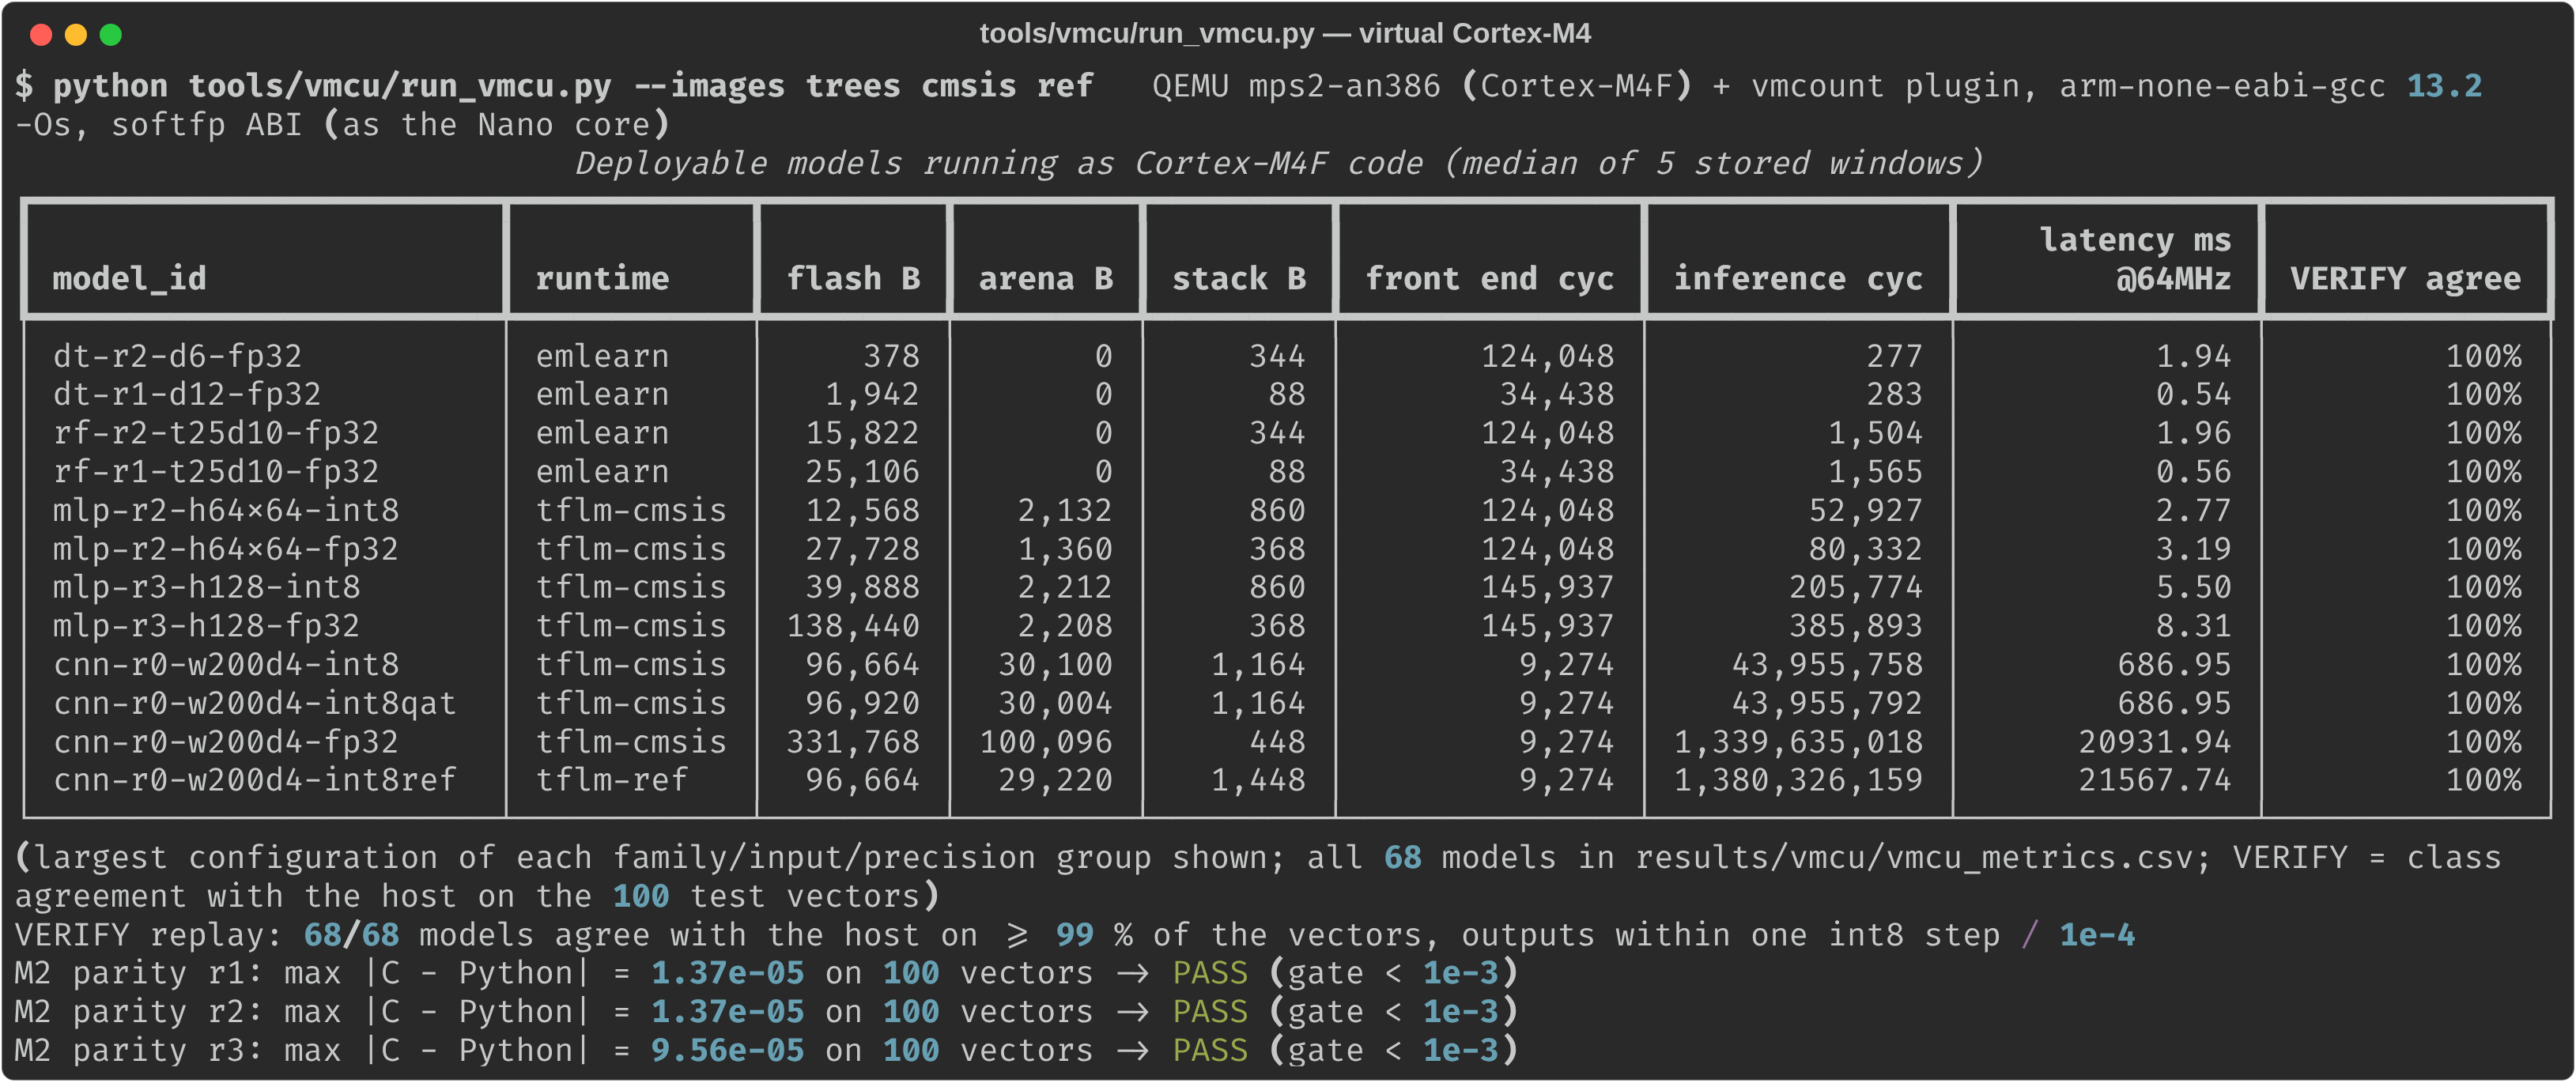
\includegraphics[width=\textwidth]{vmcu_run}\\[2pt]
{\footnotesize (a) Virtual Cortex-M4: the deployable code of every model runs as Cortex-M4F machine code in QEMU
(largest configuration of each group shown; all 68 in \texttt{results/vmcu/vmcu\_metrics.csv}).}\\[10pt]
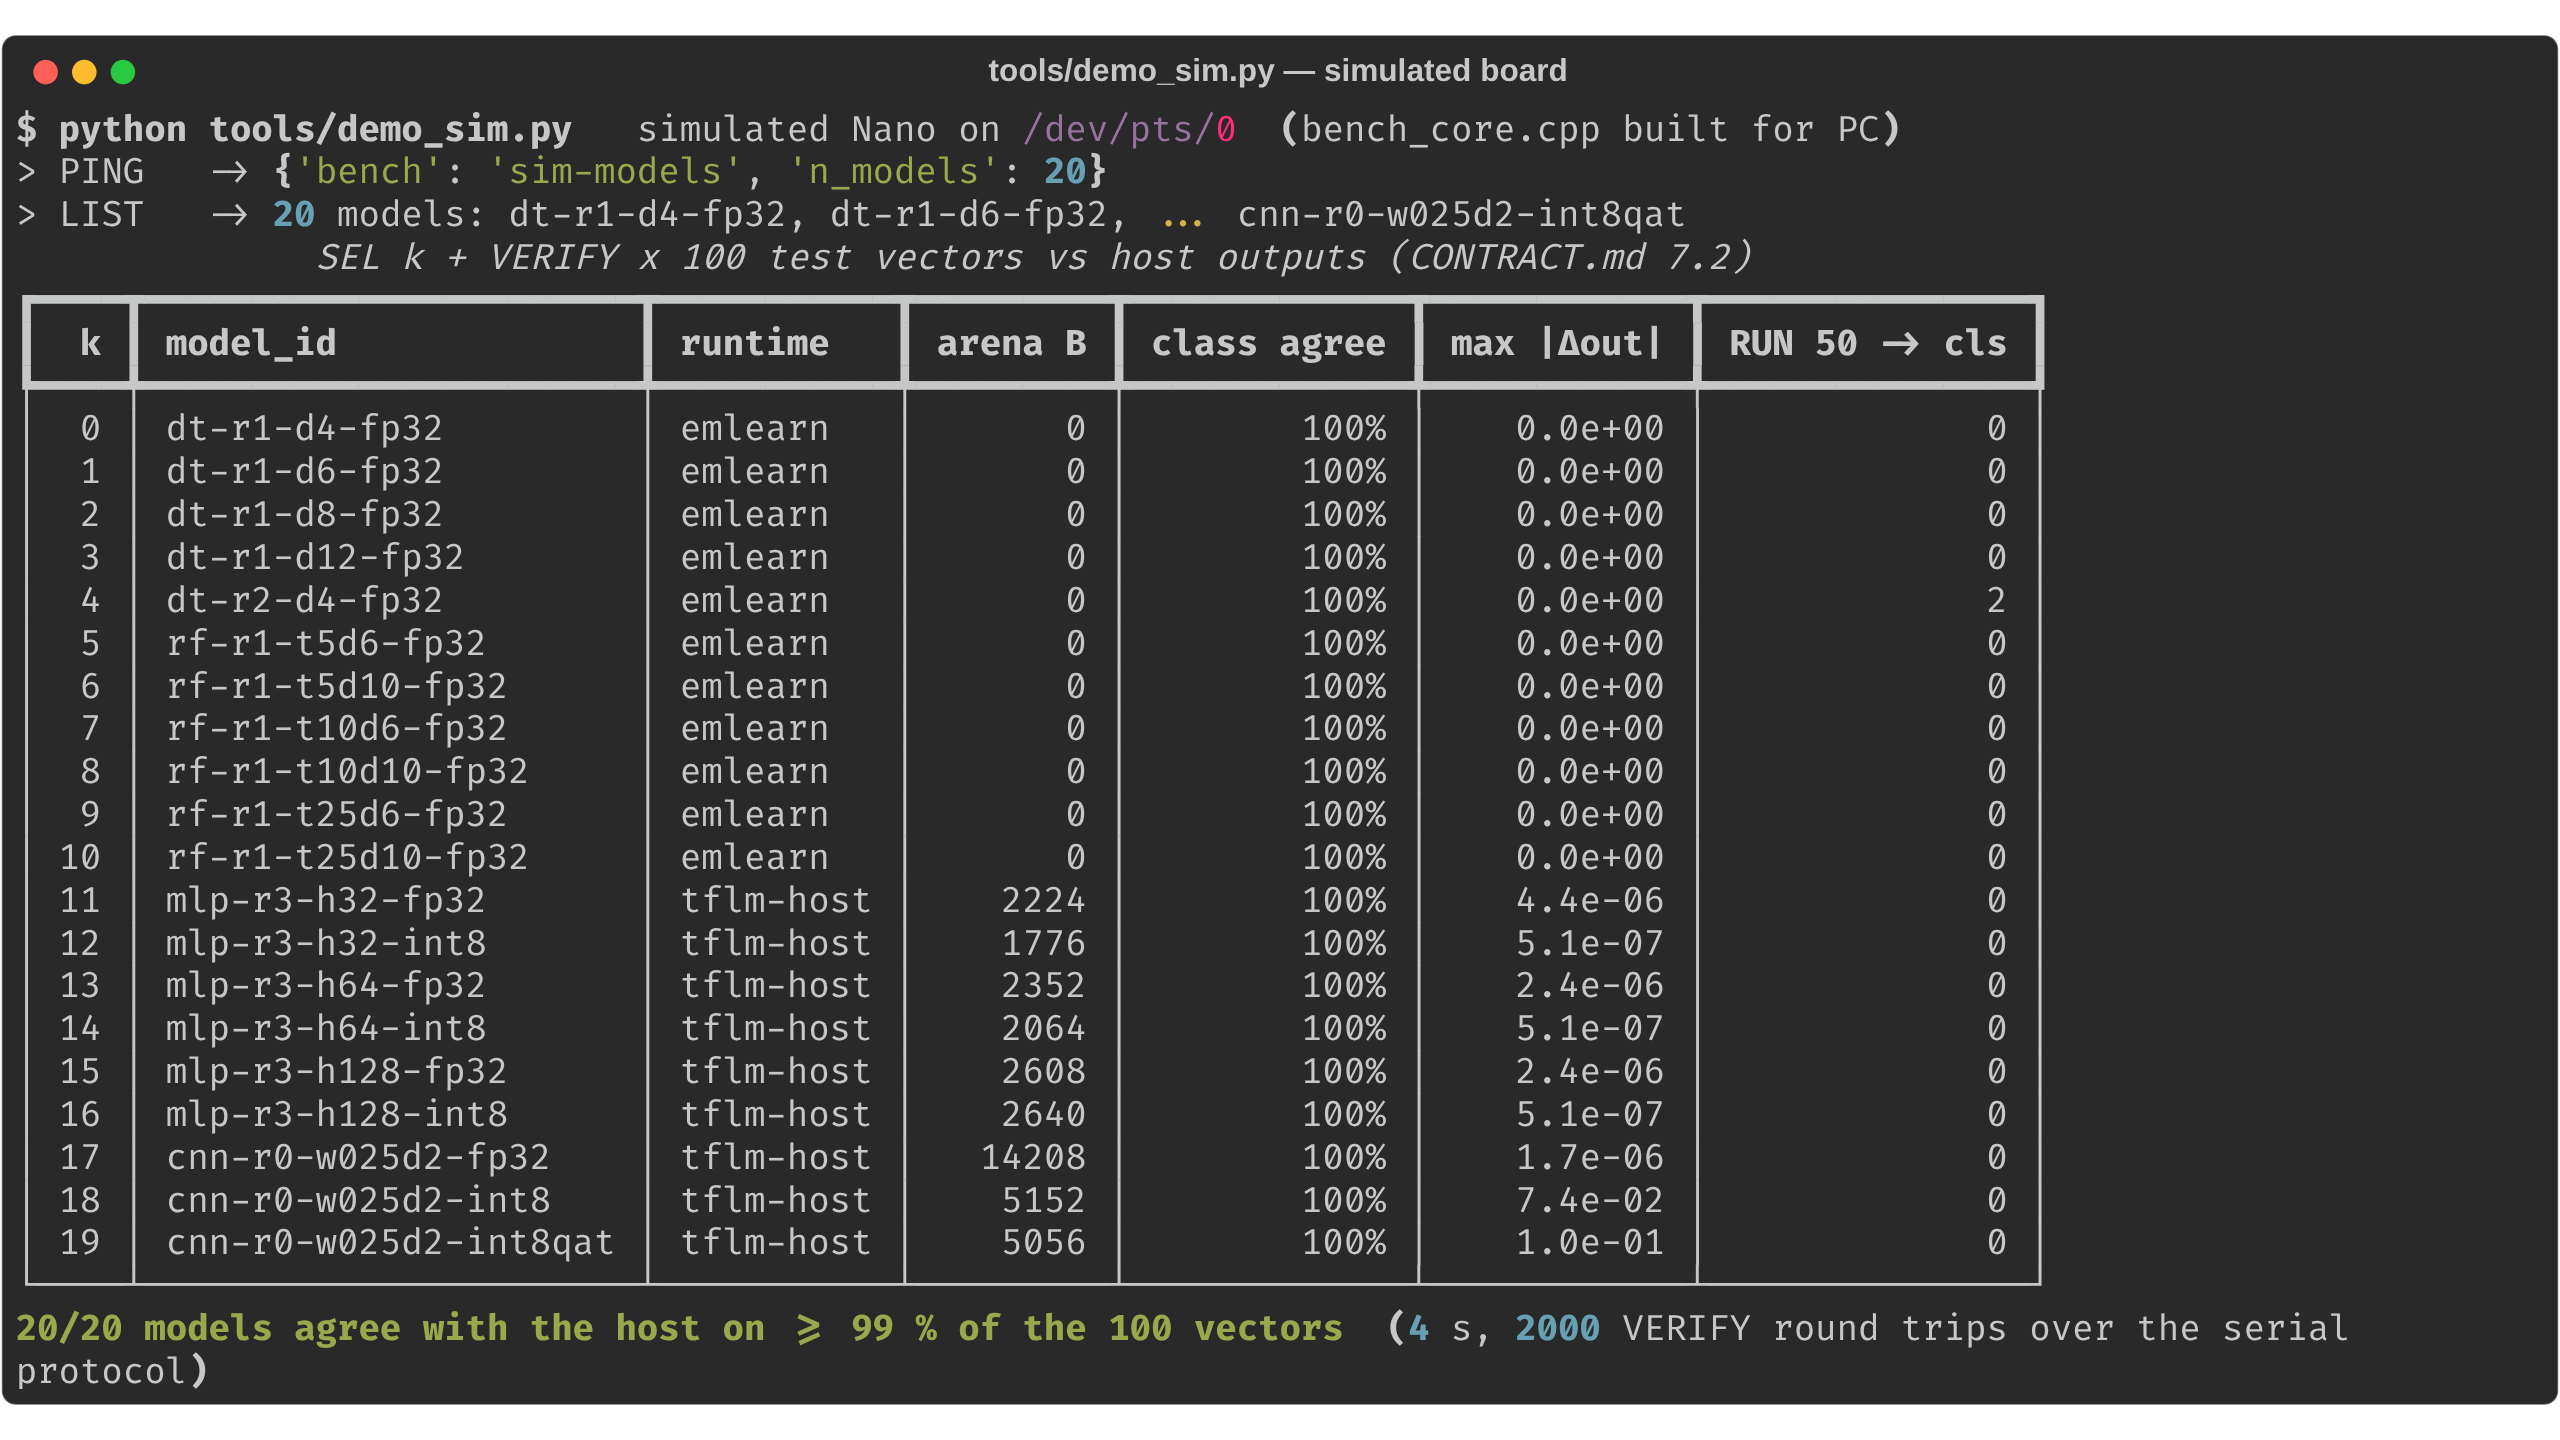
\includegraphics[width=0.82\textwidth]{demo_sim}\\[2pt]
{\footnotesize (b) Simulated board: the team's bench firmware, built for the PC with real models and the C front end,
driven over the serial protocol by \texttt{tools/dut.py} (SEL, VERIFY on the 100 test vectors, RUN).}
\caption{The two pre-hardware demonstrations. Both use the exact artefacts that will be flashed to the Nano~33~BLE.}
\label{fig:demo}
\end{figure*}

\begin{figure}[t]
\centering
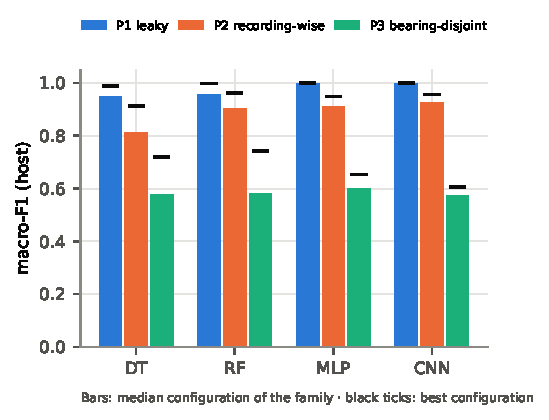
\includegraphics[width=0.86\columnwidth]{fig_protocol_drop}
\caption{Host macro-F1 per family under the three protocols (bars: median configuration; ticks: best
configuration). Mean over all folds and the seeds run so far (\NumSeedsMin{}--\NumSeedsMax{} per configuration).}
\label{fig:protocols}
\end{figure}

\subsection{Leakage changes the answer (RQ3, accuracy)}
Fig.~\ref{fig:protocols} and Table~\ref{tab:f1} summarise \NumRuns{} host runs. Under the leaky split every family
looks near-perfect (best \NumPOneBest{}). Holding out a recording (P2) costs little for the best models but separates
the families, and on unseen bearings (P3) the best model reaches only \NumPThreeBest{} macro-F1
(\NumPThreeBestModel{}), on a 4-class task. Rankings move with the protocol: Kendall's $\tau$ between the per-model
macro-F1 rankings is \NumTauModelPOnePTwo{} (P1 vs P2), \NumTauModelPOnePThree{} (P1 vs P3) and
\NumTauModelPTwoPThree{} (P2 vs P3). Bearing-disjoint scores also vary strongly across folds and seeds (standard
deviations up to \NumPThreeMLPBestStd{} in Table~\ref{tab:f1}). In this sweep, the apparent P3 winner changed
family when the MLPs went from one seed to five, so a single-seed P3 comparison is not reliable; the final
version reports every configuration over five seeds.

\begin{table}[t]
\centering
\caption{Best configuration per family: macro-F1, mean $\pm$ std over folds and seeds.}
\label{tab:f1}
\setlength{\tabcolsep}{3pt}
\begin{tabular}{lccc}
\toprule
Family & P1 leaky & P2 recording & P3 bearing \\
\midrule
DT  & \NumPOneDTBest{}$\pm$\NumPOneDTBestStd{} & \NumPTwoDTBest{}$\pm$\NumPTwoDTBestStd{} & \NumPThreeDTBest{}$\pm$\NumPThreeDTBestStd{}\\
RF  & \NumPOneRFBest{}$\pm$\NumPOneRFBestStd{} & \NumPTwoRFBest{}$\pm$\NumPTwoRFBestStd{} & \NumPThreeRFBest{}$\pm$\NumPThreeRFBestStd{}\\
MLP & \NumPOneMLPBest{}$\pm$\NumPOneMLPBestStd{} & \NumPTwoMLPBest{}$\pm$\NumPTwoMLPBestStd{} & \NumPThreeMLPBest{}$\pm$\NumPThreeMLPBestStd{}\\
CNN & \NumPOneCNNBest{}$\pm$\NumPOneCNNBestStd{} & \NumPTwoCNNBest{}$\pm$\NumPTwoCNNBestStd{} & \NumPThreeCNNBest{}$\pm$\NumPThreeCNNBestStd{}\\
\bottomrule
\end{tabular}
\end{table}

\subsection{The front end dominates feature-based models (RQ2)}
Fig.~\ref{fig:breakdown} separates the two phases on the virtual Cortex-M4. A decision tree or forest needs
\NumTreeInfMin{}--\NumTreeInfMax{} estimated cycles per window, but its R1 front end needs \NumFeROneKcyc{}\,k cycles
and its R2 front end (statistics plus a 1024-point FFT) \NumFeRTwoKcyc{}\,k: at least \NumTreeFeShareMin{} of the
end-to-end work. R0 normalisation for CNNs costs \NumFeRZeroKcyc{}\,k cycles. Counting the front end therefore moves
every feature-based model by two orders of magnitude on the energy axis, while CNNs barely move
(Fig.~\ref{fig:rq2}). This is the effect that inference-only reporting hides.

\begin{figure}[t]
\centering
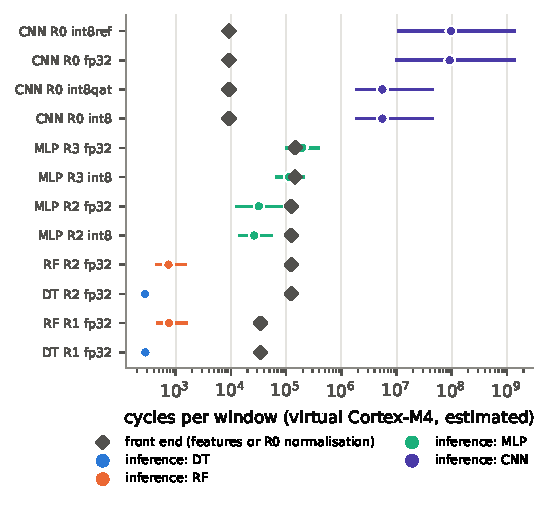
\includegraphics[width=0.86\columnwidth]{fig_energy_breakdown}
\caption{Front-end versus inference cycles per window on the virtual Cortex-M4 (median over configurations; bars
span the configurations of a group). Log scale.}
\label{fig:breakdown}
\end{figure}

\subsection{Frontiers and family dominance (RQ1, RQ3)}
Fig.~\ref{fig:pareto} shows error against estimated end-to-end energy under P2 and P3. With three objectives
(error, energy, peak RAM), the P2 frontier holds \NumFrontPTwoEtoe{} models (\NumRobustPTwoEtoe{} with bootstrap
membership probability $\geq 0.5$) and the P3 frontier \NumFrontPThreeEtoe{} (\NumRobustPThreeEtoe{}). The bootstrap
resamples test windows and draws each model's energy inside its cycle-model band (\NumBandMin{}--\NumBandMax{} wide),
so membership reflects both accuracy noise and cost-model uncertainty. Ranked by hypervolume, the families order as
\NumRankPOne{} under P1, \NumRankPTwo{} under P2 and \NumRankPThree{} under P3 (Kendall $\tau$ =
\NumTauFamPOnePTwo{}, \NumTauFamPOnePThree{} and \NumTauFamPTwoPThree{} for P1--P2, P1--P3 and P2--P3).

\begin{figure*}[t]
\centering
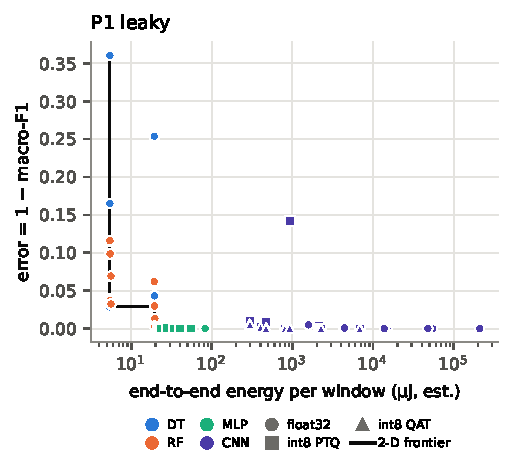
\includegraphics[width=0.32\textwidth]{fig_pareto_P1_e2e}\hfill
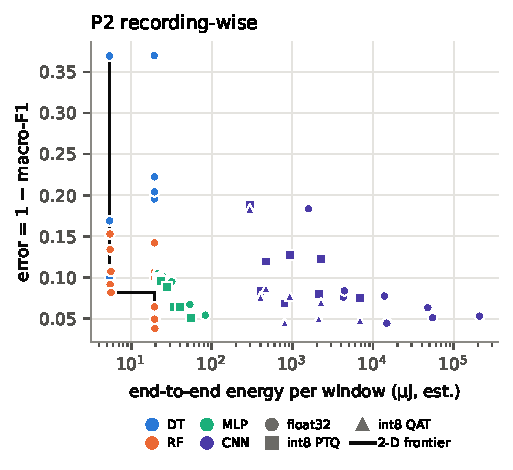
\includegraphics[width=0.32\textwidth]{fig_pareto_P2_e2e}\hfill
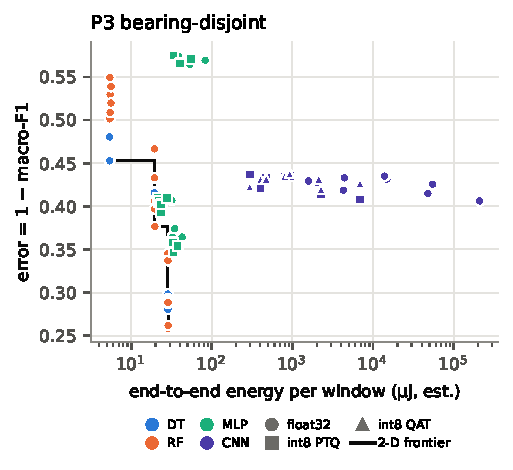
\includegraphics[width=0.32\textwidth]{fig_pareto_P3_e2e}
\caption{Error versus estimated end-to-end energy per window for every deployable configuration under P1, P2 and P3.
Colour: family; marker: precision; black staircase: two-dimensional frontier.}
\label{fig:pareto}
\end{figure*}

\begin{figure}[t]
\centering
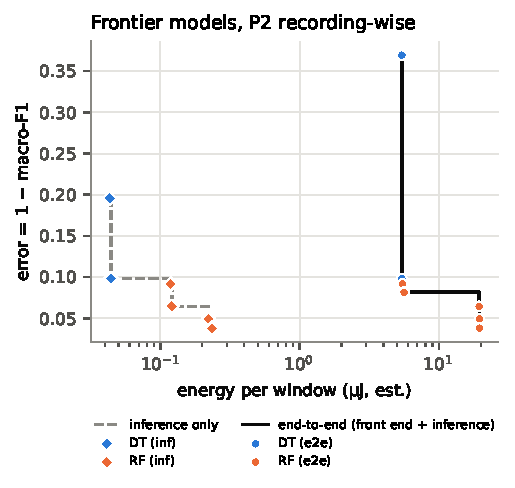
\includegraphics[width=0.86\columnwidth]{fig_rq2_frontend}
\caption{Accuracy--energy frontier members under P2 with inference-only (diamonds, dashed) and end-to-end energy
(circles, solid).}
\label{fig:rq2}
\end{figure}

\begin{table*}[t]
\centering
\caption{Pre-hardware cost on the virtual Cortex-M4 (64\,MHz, estimated) and host macro-F1 of the best P3 configuration in each family/input/precision group.}
\label{tab:costs}
\setlength{\tabcolsep}{4pt}
\begin{tabular}{lrrrrrrccc}
\toprule
Configuration & Flash (kB) & Peak RAM (kB) & Front end (kcyc) & Inference (kcyc) & Latency (ms) & Energy ($\mu$J) & P1 F1 & P2 F1 & P3 F1\\
\midrule
\texttt{dt-r1-d4-fp32} & 0.3 & 0.1 & 34.4 & 0.3 & 0.54 & 5.4 & 0.640 & 0.631 & 0.547\\
\texttt{rf-r1-t5d6-fp32} & 2.8 & 0.1 & 34.4 & 0.5 & 0.55 & 5.4 & 0.884 & 0.847 & 0.499\\
\texttt{dt-r2-d6-fp32} & 0.4 & 8.5 & 124.0 & 0.3 & 1.94 & 19.4 & 0.957 & 0.804 & 0.584\\
\texttt{rf-r2-t25d6-fp32} & 7.6 & 8.5 & 124.0 & 1.4 & 1.96 & 19.6 & 0.987 & 0.951 & 0.623\\
\texttt{mlp-r2-h64-int8} & 6.1 & 10.3 & 124.0 & 26.4 & 2.35 & 23.5 & 1.000 & 0.905 & 0.607\\
\texttt{mlp-r2-h64-fp32} & 10.4 & 9.5 & 124.0 & 32.2 & 2.44 & 24.4 & 1.000 & 0.905 & 0.608\\
\texttt{mlp-r3-h64-int8} & 20.6 & 11.5 & 145.9 & 114.0 & 4.06 & 40.6 & 1.000 & 0.935 & 0.434\\
\texttt{mlp-r3-h64-fp32} & 68.4 & 11.3 & 145.9 & 196.5 & 5.35 & 53.4 & 1.000 & 0.933 & 0.435\\
\texttt{cnn-r0-w025d2-int8qat} & 4.3 & 9.5 & 9.3 & 1887.1 & 29.63 & 295.8 & 0.988 & 0.816 & 0.600\\
\texttt{cnn-r0-w025d4-int8} & 7.9 & 10.5 & 9.3 & 2564.2 & 40.21 & 401.5 & 0.999 & 0.916 & 0.613\\
\texttt{cnn-r0-w025d4-fp32} & 10.3 & 18.2 & 9.3 & 27436.5 & 428.84 & 4281.5 & 1.000 & 0.924 & 0.614\\
\texttt{cnn-r0-w025d4-int8ref} & 7.9 & 10.5 & 9.3 & 29165.0 & 455.85 & 4551.2 & 0.999 & 0.916 & 0.613\\
\bottomrule
\end{tabular}
\end{table*}


\subsection{Kernels, precision and memory}
Table~\ref{tab:costs} lists the cost and accuracy of the best bearing-disjoint configuration of every
family/input/precision group.
On the same int8 CNNs, CMSIS-NN kernels cut estimated inference cycles by \NumCmsisMin{}--\NumCmsisMax{}$\times$
(median \NumCmsisMedian{}$\times$) relative to TFLM's reference kernels (Fig.~\ref{fig:ablation}); float CNNs, which
CMSIS-NN does not accelerate, need \NumCnnFpOverIntMin{}--\NumCnnFpOverIntMax{}$\times$ the cycles of their int8
versions. For the smallest MLPs, int8 brings no speed-up, because quantising the input and requantising each layer
cost about as much as the few hundred MACs they replace. Peak RAM (arena, feature buffers and stack) ranges from
\NumRamMinB{}\,B to \NumRamMaxKB{}\,kB, and the largest model needs \NumFlashMaxKB{}\,kB of flash.

\begin{figure}[t]
\centering
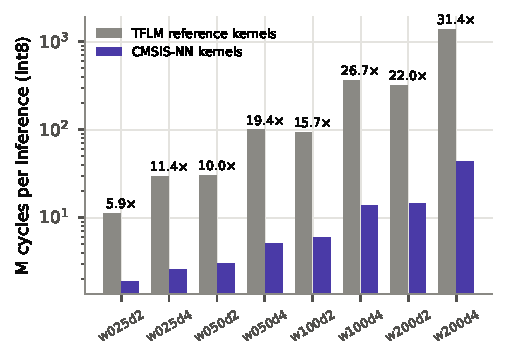
\includegraphics[width=0.86\columnwidth]{fig_cmsis_ablation}
\caption{Kernel ablation: estimated inference cycles of the int8 CNNs with TFLM reference kernels and with CMSIS-NN.}
\label{fig:ablation}
\end{figure}

\subsection{Battery life (RQ4)}
With chip-level sleep power (\SI{9.5}{\micro W}) and a CR2032 cell, the crossover rate $r^\ast$, below which sleep
dominates and the model's energy stops mattering, ranges from \NumFstarLo{}\,Hz (\NumFstarLoModel{}) to
\NumFstarHi{}\,Hz (\NumFstarHiModel{}) for the most accurate P3 model of each family (Fig.~\ref{fig:life}). At
board-level sleep power (about 3\,mW for the Nano~33~BLE), sleep dominates at every practical rate. Measuring the
board's real sleep floor is therefore part of the hardware campaign.

\begin{figure}[t]
\centering
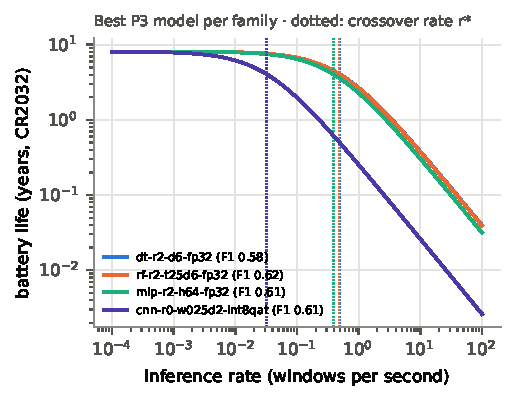
\includegraphics[width=0.86\columnwidth]{fig_lifetime}
\caption{Battery life versus inference rate for the most accurate P3 model of each family (estimated energy,
chip-level sleep). Dotted: crossover rate $r^\ast$.}
\label{fig:life}
\end{figure}

\begin{figure}[t]
\centering
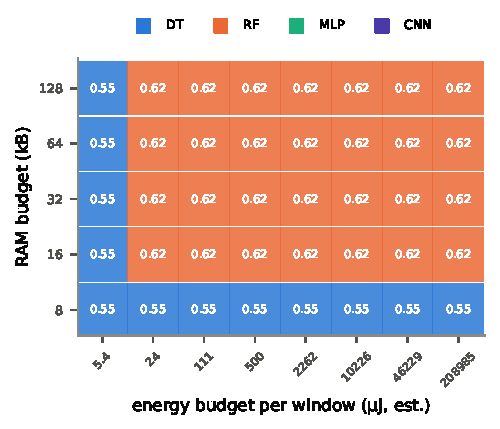
\includegraphics[width=0.8\columnwidth]{fig_rubric}
\caption{Preliminary rubric: best P3 macro-F1 (cell value) and its family (colour) under RAM and estimated-energy
budgets.}
\label{fig:rubric}
\end{figure}

\subsection{Robustness to sensor noise}
Adding white noise to the test windows separates models that clean accuracy cannot. At 0\,dB SNR under P2, the best
configuration of each family keeps a macro-F1 of \NumSnrZeroPTwoDT{} (DT), \NumSnrZeroPTwoRF{} (RF),
\NumSnrZeroPTwoMLP{} (MLP) and \NumSnrZeroPTwoCNN{} (CNN).

% =====================================================================================================================
\section{Toward a Selection Rubric}
Fig.~\ref{fig:rubric} gives the most accurate P3 model that fits each RAM and energy budget. It is the first version
of the rubric the study will deliver. The procedure: fix RAM and flash budgets; derive an energy budget from the
inference rate and the target battery life; if the rate is far below $r^\ast$, take the most accurate model that fits
RAM; otherwise take the cheapest model above the accuracy floor. Always quote bearing-disjoint (P3) accuracy, never P1.


% =====================================================================================================================
\section{Limitations and Next Steps}
This version has no board measurements. Cycles come from an instruction-exact emulator with a static Cortex-M4
timing model. Energies are proportional to cycles, so they cannot show power differences between, for example, FPU-
and integer-heavy code. The board's DWT counts (\texttt{LAT}) will calibrate the model, and
\texttt{tools/vmcu/calibrate.py} is in place for that. The INA219 rig will then replace every energy number, including
the board-level overheads (regulator, USB PHY) that the chip-level estimate omits. The virtual MCU uses current
tflite-micro and GCC~13, while the board uses Chirale's TFLM build and GCC~7, a difference the calibration will
quantify. The CNN sweep has fewer seeds than the trees so far. CWRU has a single bearing per fault class and an
artificially seeded fault, and in P3 the normal class can only be split by load. Paderborn is the planned
generalisation check.

\FloatBarrier
\section{Conclusion}
Before any hardware arrived, the full pipeline was built and gated in emulation: data, leakage-checked splits,
\NumConfigs{} deployable configurations, a virtual Cortex-M4 that runs the exact deployable code, and firmware bundles
that link for the board. The preliminary answer to the project's question is already protocol-dependent. Leaky
evaluation makes every family look interchangeable; bearing-disjoint evaluation does not. For feature-based models,
the front end, not the classifier, sets the energy cost. The hardware campaign now has to confirm these effects with
measured energy.

